\documentclass[final,5p,times]{elsarticle}

% ===================== PACKAGES =====================
\usepackage{amsmath,amssymb,amsfonts}
\usepackage{algorithmic}
\usepackage{graphicx}
\usepackage{textcomp}
\usepackage{xcolor}
\usepackage{booktabs}
\usepackage{array}
\usepackage{float}
\usepackage{url}
\usepackage{multirow}
\usepackage[utf8]{inputenc}
\usepackage{algorithm}
\usepackage{tabularx}
\usepackage{tikz}
\usepackage{pgfplots}
\pgfplotsset{compat=1.18}
\usepackage{microtype}
\usetikzlibrary{arrows.meta, positioning}

% Hyperref MUST be last
\usepackage[colorlinks=true,
linkcolor=blue,
citecolor=blue,
urlcolor=blue]{hyperref}

% ===================== JOURNAL =====================
\journal{Journal of Information Security and Applications}

\begin{document}

% ===================== FRONTMATTER =====================
\begin{frontmatter}

\title{Blockchain-Enabled Time-Lock Encryption for Academic Integrity and Secure Examination}

\author[inst1]{Sudhanshu Ranjan Dubey}
\author[inst1]{Dr. Abhinesh Kaushik}

\address[inst1]{Department of Computer Science, Indian Institute of Information Technology, Lucknow, Uttar Pradesh, India}

% ===================== ABSTRACT =====================
\begin{abstract}
The rapid migration of academic assessments to online environments has exposed deep-seated vulnerabilities in conventional examination infrastructure. A majority of existing testing platforms still rely on centralized database architectures, where a single compromised server could potentially expose student identities, enable grade manipulation, or facilitate premature leakage of question papers. The scenario of an insider gaining access to examination content hours before the scheduled start remains a persistent and largely unaddressed threat in the literature. In response to this specific class of vulnerability, we present a decentralized examination framework that couples distributed blockchain networks with Time-Lock Encryption (TLE). Rather than delegating the safekeeping of examination files to a central administrator—whose trustworthiness can never be fully guaranteed—our approach mathematically constrains the availability of decryption keys. Although students may download encrypted examination files well in advance, the cryptographic key material necessary for decryption remains computationally inaccessible until the designated examination time. The system leverages computational reference clocks together with witness encryption constructs, thereby eliminating the dependency on trusted intermediaries. Empirical evaluation of the prototype confirms robust resistance to premature content access, and the architecture exhibits sufficient scalability for deployment within large university settings. The principal contribution lies in shifting the basis of examination security from administrative oversight to verifiable cryptographic assurances.
\end{abstract}

\begin{keyword}
Blockchain \sep Time-Lock Encryption \sep Smart Contracts \sep Academic Integrity \sep Cryptography \sep Secure Examination \sep Ed-Tech \sep Witness Encryption
\end{keyword}

\end{frontmatter}

\section{Introduction}

Over the past several years, educational institutions at all levels have increasingly turned to online assessment tools for conducting examinations. The convenience these digital platforms provide is, of course, substantial—remote proctoring, automated grading, and flexible scheduling have become staples of modern pedagogy. Yet this convenience masks what we see as a rather serious set of security shortcomings. In a typical deployment, the institution stores all examination questions on a single centralized server. Should an attacker succeed in compromising that particular machine, the integrity of the entire assessment collapses \cite{chen2013security}. We would argue that this centralized storage paradigm almost invites data manipulation and denial-of-service incidents.

Among the many threats, premature leakage of examination papers arguably stands as the most corrosive. Consider the operational reality of a conventional digital examination. Encrypted copies of the question paper are often transmitted to examination centres or placed in cloud repositories hours, and sometimes days, before the test is actually administered. Throughout this interim period, there exists a non-trivial window during which malicious actors—ranging from external attackers to compromised or disgruntled staff members—could intercept the files. When sealed examination content is accessed before the designated time, the reputational and academic consequences for the institution can be devastating.

To date, the standard response from system designers has been to apply established cryptographic primitives such as RSA or Elliptic Curve Cryptography. While these techniques are mathematically sound in isolation, they do not resolve a fundamental operational weakness: some human administrator must hold, and at the right moment release, the master decryption key. If that individual commits an error, falls victim to social engineering, or is otherwise compromised, the entire cryptographic apparatus becomes moot. There is, we believe, a pressing need for examination environments in which security guarantees derive from mathematical structure rather than from assumptions about the reliability of every individual in the administrative chain.

\subsection{The Shift to Trustless Architecture}
This observation has motivated our departure from conventional database-centric models in favour of decentralized blockchain technology. At its core, a blockchain functions as a distributed ledger whose state is independently verified by thousands of participating nodes. Any attempt to retroactively alter a committed record would require an adversary to gain computational dominance over more than half the network—a task that, on established chains, is generally considered infeasible.

In this work, we put forward what we term a Blockchain-Enabled Time-Lock Encryption (BETLE) mechanism. The scheme goes beyond mere encryption of examination content; it binds the decryption process itself to the passage of real-world time. A student might hold the encrypted file on a local disk for an entire week and yet remain unable to recover the plaintext until the precise examination start time arrives. This coupling of encryption with temporal constraints addresses the leakage problem at its root, and it does so by relying on the consensus properties of public blockchains rather than on any centralised authority \cite{tschorsch2016bitcoin}.

\subsection{Using the Blockchain as a Clock}
One can think of Time-Lock Encryption as a kind of digital vault fitted with a countdown timer. Historically, implementing such a timer has always required some trusted party to guard the key and release it at the appointed hour. Blockchain technology offers a path around that requirement entirely. Public blockchains such as Ethereum produce new blocks at intervals that, while not perfectly fixed, are statistically predictable over modest time horizons. Our system exploits this regularity by using the blockchain height as what Liu et al. termed a \textit{computational reference clock} \cite{liu2018build}. The decryption key is mathematically tied to a particular future block—one that has not yet been mined. Because no participant in the network can predict the exact hash of a block before it is produced, it becomes impossible for anyone, including the system designer, to accelerate the unlocking process. In effect, the scheme transmits information into the future with cryptographic certainty.

\subsection{Automating the Administrator}
A further dimension of our design involves delegating routine administrative tasks to smart contracts—self-executing programs that reside on the blockchain and operate according to deterministic rules, free from human discretion or interference.
\begin{itemize}
    \item \textbf{Automated Verification:} The contract cross-references student wallet addresses against a pre-registered whitelist, which eliminates the possibility of manual entry errors as well as any scope for selective bias in admission to the examination.
    \item \textbf{Tamper-Proof Rules:} Once examination parameters—such as the unlock block number—are committed to the network, they become immutable. If, for instance, a test is programmed to unlock at block 150000, no entity can bring that moment forward.
    \item \textbf{Permanent Logging:} Each student submission produces a cryptographic hash that is recorded on-chain, creating an indelible audit trail. This record is beyond post-hoc modification, a property that directly addresses concerns raised in earlier work on result tampering \cite{samanta2021blockchain}.
\end{itemize}

\subsection{Economic and Operational Efficiency}
The benefits of this architectural shift extend beyond security alone. Al Hemairy et al. \cite{AlHemairy2024} noted that decentralized frameworks can substantially reduce the costs traditionally incurred through physical logistics, secure printing of question papers, and the deployment of human proctors at examination centres. When distribution and verification are handled through smart contracts—a model that is also gaining traction in the context of secure university admissions \cite{mori2020digital}—the operational overhead of administering high-stakes assessments drops appreciably, while institutional trust in the certification pipeline arguably strengthens. To give a rough sense of scale, mid-sized universities routinely spend non-trivial sums on printing and courier services for examination materials each year; a verifiable digital distribution model could reclaim a significant portion of that expenditure.

The remainder of this paper is organised as follows. We discuss the mathematical underpinnings of Witness Encryption and Time-Lock Puzzles, describe the system architecture built around the InterPlanetary File System (IPFS) for off-chain storage, and present empirical results pertaining to transaction throughput and gas consumption on the Ethereum network.

\section{Literature Review}

Over the past decade or so, electronic testing environments have matured considerably—from rudimentary password-protected PDF distributions to elaborate, multi-layered security ecosystems that may incorporate biometric scanners, encrypted communication channels, and decentralized storage networks. In situating the BETLE architecture within this evolving landscape, we surveyed a range of foundational and recent contributions.

\subsection{Blockchain-Based Examination Systems}
Distributed ledger technology has attracted growing interest among researchers concerned with the integrity of university assessment processes. Samanta et al. \cite{samanta2021blockchain}, for example, implemented a system on Hyperledger Fabric with the explicit aim of addressing the lack of transparency in conventional grading workflows. Their central argument—that centralized SQL databases leave grade records exposed to quiet, internal modification—is well taken. An administrator who decides to adjust a student's mark in a standard relational database may leave no trace that any change occurred. By committing final grades to a private blockchain, Samanta's team introduced a requirement for network-wide consensus before any record could be altered.

That said, their system is designed primarily to protect the \textit{post-examination} phase: the storage of results and the issuance of credentials against forgery. Acharya and Binu \cite{acharya2018blockchain} similarly concentrated on blockchain-backed record maintenance, though again with a focus squarely on grade storage. A recent systematic review by Farooq et al. \cite{farooq2021blockchain} corroborates what we observed in our own survey—namely, that although numerous assessment-oriented blockchain models have been proposed, very few grapple seriously with real-time integrity during the question distribution phase. Sultana et al. \cite{sultana2024proposed}, in one of the more recent contributions, proposed blockchain-based improvements to examination reliability, but the pre-examination leakage window remains outside the scope of their work. Our research is aimed precisely at this gap: devising a mechanism for the secure, temporally controlled delivery of question papers, prior to any grading activity.

\subsection{Biometric Authentication and Access Control}
The well-documented fragility of password-based authentication makes it a poor fit for high-stakes testing. Students routinely share login credentials, rendering conventional username-and-password gates all but ceremonial. Zhu and Cao \cite{zhu2021secure} addressed this by constructing a framework that fuses facial recognition with a blockchain backend. They employed a ``Fuzzy Vault'' approach to protect the stored biometric templates; even in the event of a database breach, reconstructing usable facial data from the vault contents would be computationally prohibitive.

For access control, their system relies on Attribute-Based Encryption (ABE). Under ABE, examination files are encrypted such that only users possessing a specific set of digital attributes—say, ``Enrolled in Math 101''—can perform decryption. This represents a meaningful improvement in preventing unauthorized access. However, it leaves an important dimension unaddressed: temporal control. Should a compromised or dishonest administrator choose to distribute decryption credentials to enrolled students several days ahead of the examination, the ABE mechanism offers no safeguard. It governs \textit{who} may open the file, but is entirely silent on \textit{when} they may do so.

\subsection{Foundations of Time-Lock Encryption}
The idea of cryptographically transmitting information ``into the future'' was first articulated in a formal setting by Rivest, Shamir, and Wagner \cite{rivest1996time}. For many years, the concept remained largely theoretical, but more recent developments have brought it closer to practical deployment, particularly in blockchain contexts. Liu et al. \cite{liu2018build}, in their work titled ``How to Build Time-Lock Encryption,'' put forward a construction that dispenses with trusted third parties altogether. Central to their proposal is the notion of a \textit{Computational Reference Clock (CRC)}.

Their argument proceeds from the observation that modelling real-world time within a cryptographic protocol is inherently difficult if one must rely on a trusted time server. As an alternative, they proposed treating the state of a public, iterative computation—concretely, the Bitcoin blockchain—as the clock itself. Because producing each new block demands a verifiable and substantial quantity of computational work under the Proof-of-Work paradigm, the blockchain height functions as a tick-tock mechanism that no single adversary can accelerate. Liu et al. then combined this clock with \textit{Witness Encryption}, a construct in which a ciphertext can be recovered only by an entity that possesses a witness satisfying a specified condition (for instance, ``knowledge of a block at height $H$''). It is this theoretical framework that supplies the mathematical foundation for our proposed solution, and it represents a significant step toward bridging the gap between abstract cryptographic constructions and the concrete demands of examination security.

\subsection{Secure E-Voting Parallels}
There is a well-recognised overlap between the security requirements of electronic voting and those of secure examinations; both domains demand anonymity, eligibility verification, and receipt-freeness. Chatterjee et al. \cite{chatterjee2023efficient} proposed an e-voting protocol built around Elliptic Curve Cryptography (ECC) and blind signatures, with a particular emphasis on keeping the cryptographic overhead low enough for deployment on mobile devices.

In their scheme, blind signatures serve to decouple the voter's identity from the content of their ballot, preserving anonymity during tallying. An analogous requirement surfaces in examinations: ideally, the grading process should be anonymous (i.e., blind marking) to minimise evaluator bias. Although our present work concentrates on the secure delivery of question papers rather than on the grading pipeline, the cryptographic primitives discussed by Chatterjee et al.—ECC and blind signatures—are pertinent to the student authentication and submission anonymity modules we envision for future iterations. It is also worth noting that Uddin et al. \cite{9498566} explored a blockchain-based e-voting architecture employing Time-Lock Encryption to keep ballots sealed until the tallying phase, which lends further support to the viability of TLE in time-sensitive, security-critical workflows.

\subsection{Smart Contracts and Privacy}
Kosba et al. \cite{7546538} introduced ``Hawk,'' a framework designed to enable privacy-preserving smart contracts. They drew attention to a tension that is often overlooked: blockchains provide transparency by design, yet that very transparency can become a liability when the data being processed is sensitive—examination answers being a prime example. Hawk offers programmers a way to compose private smart contracts without having to implement the underlying cryptographic mechanisms from scratch. In a complementary direction, Peng et al. \cite{zeroknowledgeproof} surveyed Zero-Knowledge Proofs (ZKPs) in the context of verifiable machine learning. Their findings suggest an intriguing possibility for future examination platforms: a student could prove, via a ZKP, that they achieved a particular performance level without disclosing their actual answers on-chain.

\subsection{Recent Advancements in Examination Workflows}
Several more recent proposals deserve mention, though each has notable limitations. Ahmed and Nagaraj \cite{npl1} employ a private blockchain with AES-128 encryption; while functional, the reliance on a centralized administrator for key management constrains the security guarantees the system can actually offer. Anuradha et al. \cite{npl2} and Jacob et al. \cite{npl3} each introduced blockchain-backed frameworks that make use of cryptographic hashing and IPFS for storage, but neither incorporates temporal access control tied to consensus-level timestamps. The framework proposed by Pranathi et al. \cite{npl5} does incorporate time-locked smart contracts, but these operate at the application layer and are therefore susceptible to certain classes of smart contract exploits. On the more theoretical side, Lai et al. \cite{lai2019fully} developed a fully decentralized TLE system whose construction underscores the inherent difficulty of achieving robust time-locks without a central authority. Li et al. \cite{li2024send} have investigated what they call blockchain-based ``time machines'' for the controlled release of locked information, although the applicability of their approach to the specific operational constraints of high-stakes university examinations has not been thoroughly explored. Importantly, none of these systems offer comprehensive security validation or wallet-based non-repudiation mechanisms for student submissions.

\subsection{Relevant Patent Literature}
A number of granted patents and published applications touch on blockchain-based security mechanisms that are at least partially relevant here. These include patents describing time-controlled token distribution \newline(US20190347656A1 \cite{us20190347656a1}), credential verification \newline(US20200234303A1 \cite{us20200234303a1}), decentralized education platforms (US20210342858A1 \cite{us20210342858a1}), secure data storage (US20190266587A1 \cite{us20190266587a1}), and blockchain-mediated authentication (US20180225651A1 \cite{us20180225651a1}). Upon closer examination, however, these disclosures are oriented primarily toward passive credential verification or general-purpose storage solutions. None of them addresses the specific problem of enforcing temporal access restrictions on examination content through consensus-level timestamp validation.

\subsection{Identified Research Gap}
Taken together, the literature reveals a persistent gap. Credential-oriented systems such as those described by Al Hemairy et al. \cite{AlHemairy2024} and biometric-focused architectures like that of Zhu and Cao \cite{zhu2021secure} each address important facets of examination security, but no existing framework—so far as we have been able to determine—integrates all three of the following capabilities:
\begin{enumerate}
    \item \textbf{Decentralized Storage:} Eliminating server-level single points of failure and reducing the blast radius of any individual compromise.
    \item \textbf{Time-Lock Encryption:} Providing a mathematical guarantee that examination content cannot be accessed prior to the scheduled start, regardless of insider cooperation.
    \item \textbf{Smart Contract Automation:} Removing the need for administrative trust during the examination lifecycle and enforcing fairness through deterministic on-chain logic.
\end{enumerate}
The BETLE system presented in this paper is our attempt to address this gap in a unified and practically deployable manner.

\section{Novel Technical Contributions}
The system has been designed with specific vulnerability classes in mind, each identified through our review of existing testing software and the literature surveyed above. The following points summarise how the BETLE architecture differentiates itself:
\begin{enumerate}
    \item \textbf{Consensus-Level Time-Locks:} Rather than relying on a server-side clock—which any sufficiently privileged insider could manipulate—our scheme anchors the examination unlock event to the blockchain's own consensus timestamps (\texttt{block.timestamp}). Advancing the release time would require an adversary to gain majority control over the mining or validating network, a proposition that is generally regarded as infeasible on established public chains.
    \item \textbf{Hybrid Encryption Pipeline:} Examination PDFs, which can be large, are processed through a two-stage encryption pipeline. The bulk content is encrypted with AES-256 in CBC mode, while the resulting symmetric keys are themselves protected with RSA-2048-OAEP. This layered approach provides a substantial security margin for the kind of content typically found in academic assessments.
    \item \textbf{Dual-Layer Immutability:} Upon upload, each examination file produces a unique Content Identifier (CID) within the InterPlanetary File System (IPFS). This CID is subsequently committed to the Ethereum blockchain, yielding two independent, mathematically verifiable proofs that the document has not been tampered with since its original submission.
    \item \textbf{Wallet-Based Authentication:} Examination submissions are signed with the student's cryptographic wallet key, which accomplishes two things simultaneously: it authenticates the submitter's identity and it creates a non-repudiable record—the student cannot plausibly claim, after the fact, that they did not submit the work.
    \item \textbf{Comprehensive Security Validation:} We evaluated the framework against 24 distinct attack vectors, with particular attention to timestamp drift manipulation and replay attacks. The results, detailed in Section VII, demonstrate a high degree of resilience.
    \item \textbf{Cost-Optimized Architecture:} On-chain execution is notoriously expensive. To mitigate this, we structured the smart contract logic around batch processing and event-based logging, which together bring the per-operation gas costs down to levels that are comfortably sustainable for institutional budgets.
\end{enumerate}

\section{System Architecture}

The BETLE framework is realised as a multi-layered decentralized application (DApp). The guiding design principle throughout has been the elimination of single points of failure. By distributing responsibilities across distinct cryptographic and storage layers, the architecture ensures that no single actor—whether the university dean, an IT systems administrator, or any other stakeholder—holds unilateral control over any phase of the examination lifecycle.

\begin{figure*}[htbp]
\centering
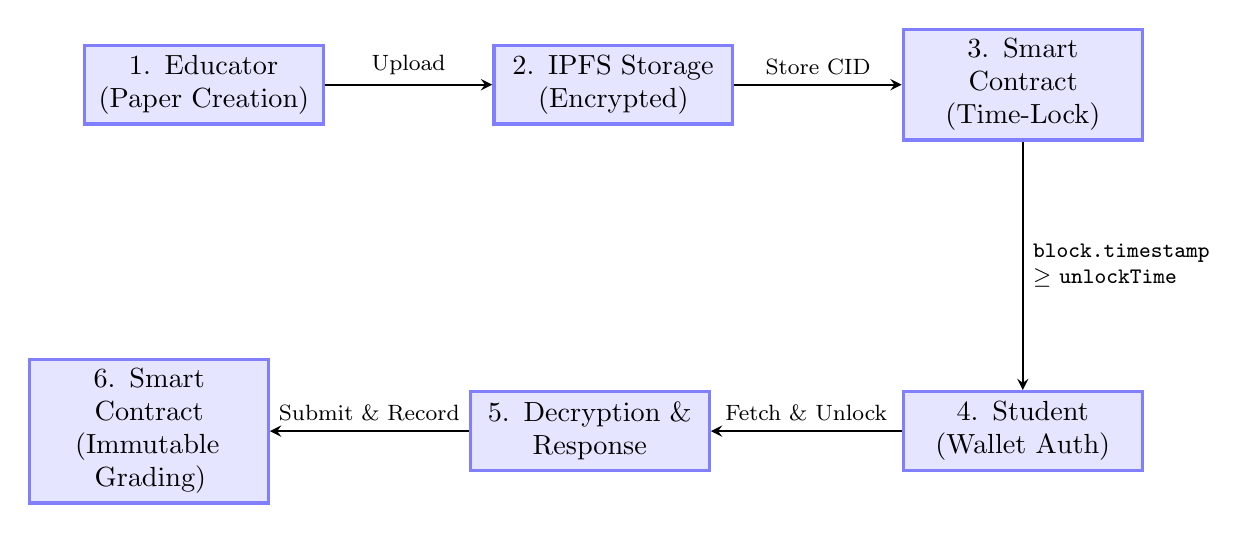
\begin{tikzpicture}[
  node distance=2.2cm,
  box/.style={rectangle, draw=blue!50, fill=blue!10, very thick, minimum width=3cm, minimum height=1cm, align=center, text width=2.8cm},
  arrow/.style={thick,->,>=stealth}
]
\node[box] (educator) {1. Educator \\ (Paper Creation)};
\node[box, right of=educator, xshift=3cm] (ipfs) {2. IPFS Storage \\ (Encrypted)};
\node[box, right of=ipfs, xshift=3cm] (sc) {3. Smart Contract \\ (Time-Lock)};
\node[box, below of=sc, yshift=-2.2cm] (student) {4. Student \\ (Wallet Auth)};
\node[box, left of=student, xshift=-3.3cm] (decrypt) {5. Decryption \& \\ Response};
\node[box, left of=decrypt, xshift=-3.4cm] (grade) {6. Smart Contract \\ (Immutable Grading)};

\draw[arrow] (educator) -- node[midway, above, font=\footnotesize] {Upload} (ipfs);
\draw[arrow] (ipfs) -- node[midway, above, font=\footnotesize] {Store CID} (sc);
\draw[arrow] (sc) -- node[midway, right, align=left, font=\footnotesize] {\texttt{block.timestamp} \\ $\ge$ \texttt{unlockTime}} (student);
\draw[arrow] (student) -- node[midway, above, font=\footnotesize] {Fetch \& Unlock} (decrypt);
\draw[arrow] (decrypt) -- node[midway, above, font=\footnotesize] {Submit \& Record} (grade);
\end{tikzpicture}
\caption{Proposed Methodology Flowchart illustrating the end-to-end examination lifecycle.}
\label{fig:methodology_flowchart}
\end{figure*}

\subsection{Architectural Layers}
The system is organised into four functionally distinct layers, each depicted in Fig. \ref{fig:System Architecture Overview}:

\begin{enumerate}
    \item \textbf{User Interface Layer:} This is the frontend web application through which students and examiners interact with the platform. It is responsible for capturing biometric data where applicable and for rendering the examination interface.
    \item \textbf{Application Logic Layer:} Sitting behind the interface, this layer processes authentication requests and mediates all interactions with the blockchain. It houses the \textit{Time-Lock Encryption Module}, which performs the cryptographic wrapping of examination papers according to the algorithms described in Section V.
    \item \textbf{Blockchain Layer:} Deployed on the Ethereum network, this layer contains the core smart contract logic governing examination scheduling, student whitelisting, and the controlled release of decryption keys at the designated block timestamp.
    \item \textbf{Storage Layer:} Storing large binary files directly on-chain would be prohibitively expensive. Accordingly, bulky artefacts—encrypted question paper PDFs, student answer scripts, and the like—are persisted on the InterPlanetary File System (IPFS). The blockchain stores only the corresponding Content Identifiers (CIDs), which serve as tamper-evident pointers to the off-chain content.
\end{enumerate}

\begin{figure}
    \centering
    \includegraphics[width=1.0\linewidth]{overview_diagram.png}
    \caption{System Architecture Overview}
    \label{fig:System Architecture Overview}
\end{figure}

\begin{figure}
    \centering
    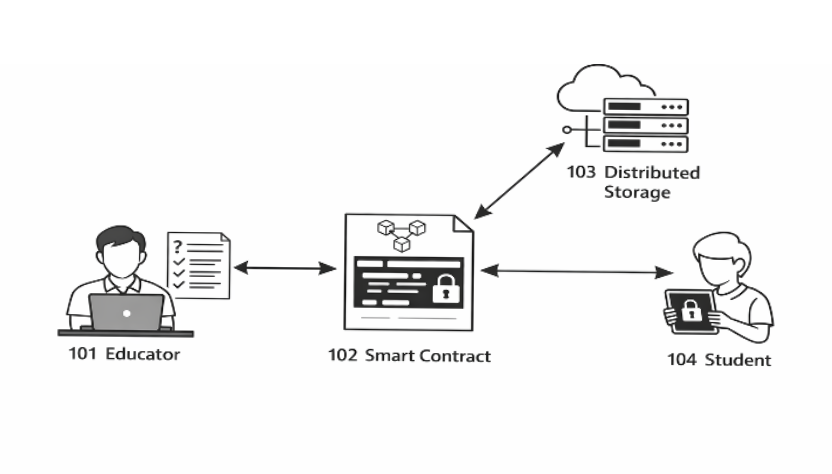
\includegraphics[width=1.0\linewidth]{Picture 1.png}
    \caption{Detailed System Workflow}
    \label{fig:Picture1}
\end{figure}

\subsection{Stakeholders in the Ecosystem}
\begin{itemize}
    \item \textbf{Administrator/Examiner:} The examiner is responsible for the initial configuration. They draft the questions, encrypt and upload the document to IPFS, and encode the precise start time ($T_{start}$) along with the permitted duration ($D$) into the smart contract. Once the transaction is confirmed, the examiner's ability to modify or prematurely release the document is revoked by the protocol itself.
    \item \textbf{Student:} Each examinee authenticates via a cryptographic wallet. Students may retrieve the encrypted file in advance and store it locally, but the contents remain inaccessible until the blockchain timestamp reaches $T_{start}$.
    \item \textbf{Verifier:} Because the underlying ledger is publicly readable, any external auditor—or, indeed, a simple automated monitoring script—can independently confirm that the examination materials were neither altered nor released ahead of schedule. This open verifiability contributes meaningfully to institutional transparency.
\end{itemize}

\section{Mathematical Methodology}

The cryptographic core of the BETLE framework rests on the application of Time-Lock Encryption (TLE). We adapted the classic puzzle construction due to Rivest, Shamir, and Wagner (RSW), and extended it with modern Witness Encryption techniques \cite{tle}. The overarching objective is to bind the accessibility of encrypted data not merely to possession of a secret key, but to the irreversible passage of time itself.

\subsection{Time-Lock Puzzle Formulation}
Conventional symmetric encryption can, in principle, be broken if an adversary is willing to devote sufficient computational resources. The construction we adopt here sidesteps that concern in a rather different way. The message $M$—which in our application contains the symmetric key that ultimately unlocks the examination paper—is rendered unrecoverable until a precisely determined number of modular squaring operations has been completed in strict sequence. The critical property of this mathematical structure is its inherently sequential nature: the squarings cannot be parallelised. No matter how powerful the hardware—whether a top-of-the-line GPU cluster or an extensive cloud computing deployment—the computation must proceed one step at a time. This forces any entity attempting premature decryption to expend a specific and non-negotiable quantity of wall-clock time.

Let $T$ be the time parameter (representing the number of squarings required).
Let $N = p \times q$ be the product of two large prime numbers $p$ and $q$.
Let $a$ be a random base.

The puzzle is generated as follows:
\begin{enumerate}
    \item The examiner calculates:
    \begin{equation}
    b = a^{2^T} \pmod N
    \end{equation}
    However, the examiner knows $\varphi(N) = (p-1)(q-1)$, so they can compute $e = 2^T \pmod{\varphi(N)}$ efficiently, then $b = a^e \pmod N$.
    \item The symmetric key $k$ is derived from $b$:
    \begin{equation}
    k = \text{Hash}(b)
    \end{equation}
    \item The exam paper $M$ is encrypted using $k$:
    \begin{equation}
    C_{paper} = \text{AES}_k(M)
    \end{equation}
    \item The examiner publishes the puzzle tuple $(N, a, T, C_{paper})$.
\end{enumerate}

\subsection{Decryption Process}
At the designated examination time, the student's client software must recover the key $k$ by solving the puzzle directly. Crucially, the student's machine does not possess the original prime factors $p$ and $q$, and therefore has no access to the Euler totient $\varphi(N)$. Without this shortcut, the software is compelled to execute all $T$ sequential squarings as specified:
\begin{equation}
W_0 = a
\end{equation}
\begin{equation}
W_{i+1} = W_i^2 \pmod N \quad \text{for } i = 0 \text{ to } T-1
\end{equation}
Finally, $b = W_T$. The key $k$ is then reconstructed as $k = \text{Hash}(b)$, allowing decryption of $C_{paper}$.

\subsection{Blockchain Integration}
Relying solely on local computation to enforce the time delay introduces an obvious fairness concern: hardware heterogeneity means that a student equipped with a high-performance workstation would complete the squarings somewhat faster than one using a modest laptop. To ensure a level playing field across all examinees, we offload the temporal enforcement to the blockchain network itself. Specifically, we use the block timestamp as a universal, consensus-validated reference clock.

The Smart Contract logic is as follows:
\begin{itemize}
    \item \textbf{Input:} \text{storePaper(ipfsHash, unlockTime)}.
    \item \textbf{Condition:} The contract stores \texttt{ipfsHash} and \texttt{unlockTime}.
    \item \textbf{Access:} When a student requests the paper, the contract checks:
    \begin{equation}
    \text{block.timestamp} \geq \text{unlockTime}
    \end{equation}
    \item \textbf{Output:} If true, the contract emits an event with the decryption key or allows the download of the key file.
\end{itemize}

\section{Algorithms and Implementation}

The practical realisation of the BETLE framework centres on two complementary algorithms: one governing the initial encryption of examination content by the examiner, and a second handling the subsequent decryption and verification on the student's side.

\subsection{Encryption Algorithm}
Algorithm 1 formalises the procedure for locking the examination paper. In our deployment, this computation is performed off-chain within the examiner's client application; only the resulting ciphertext hash and associated metadata are committed to the blockchain, which keeps gas expenditure to a minimum. The corresponding workflow is depicted in Figure \ref{fig:Picture3}.

\begin{figure}[htbp]
    \centering
    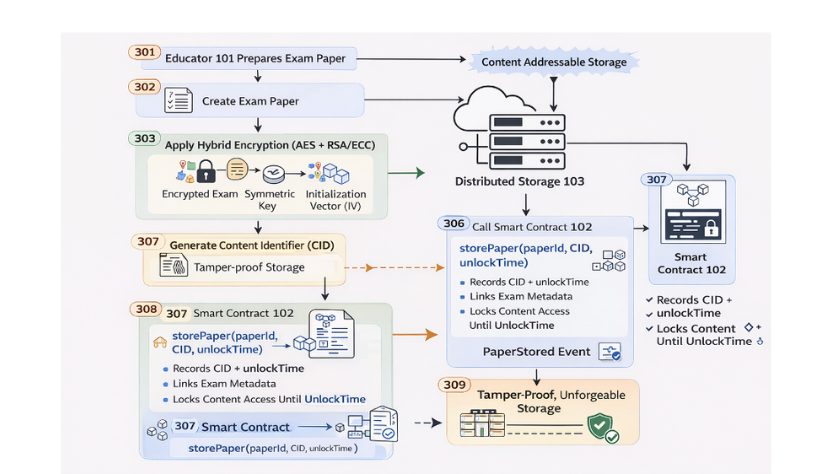
\includegraphics[width=1.0\linewidth]{Picture 3.png}
    \caption{Flowchart of Examination paper encryption and storage}
    \label{fig:Picture3}
\end{figure}

\begin{algorithm}[H]
\caption{Time-Lock Puzzle Encryption (RSW Scheme)}
\label{alg:encryption}
\begin{algorithmic}[1]
\REQUIRE Message $M$, time parameter $T$, modulus $N=pq$, base $a$
\ENSURE Ciphertext tuple $(C, a, T, N)$
\STATE Compute $b \leftarrow a^{2^T} \pmod N$ \COMMENT{Using Euler's Totient shortcut}
\STATE Compute symmetric key $k \leftarrow \text{Hash}(b)$
\STATE Encrypt message: $C \leftarrow \text{AES}_k(M)$
\RETURN $(C, a, T, N)$
\end{algorithmic}
\end{algorithm}

\subsection{Decryption Algorithm}
Algorithm 2 formalises the unlocking procedure. Within the Witness Encryption model we adopt, the release of the key is conditioned on the network's miners (or validators) confirming that the current block height or timestamp satisfies the pre-specified threshold before the key-release transaction can be validated.

\begin{algorithm}[H]
\caption{Time-Lock Puzzle Decryption}
\label{alg:decryption}
\begin{algorithmic}[1]
\REQUIRE Ciphertext $(C, a, T, N)$
\ENSURE Plaintext message $M$
\STATE Compute $b \leftarrow a^{2^T} \pmod N$ \COMMENT{Sequential computation required by solver}
\STATE Compute decryption key $k \leftarrow \text{Hash}(b)$
\STATE Decrypt message: $M \leftarrow \text{AES}_k^{-1}(C)$
\RETURN $M$
\end{algorithmic}
\end{algorithm}

\section{Performance Evaluation}

To assess the performance, scalability, and economic viability of the proposed system, we deployed it on an Ethereum Testnet (Sepolia/Goerli) and carried out a series of controlled experiments. The test environment comprised the following:
\begin{itemize}
    \item \textbf{Hardware:} AMD FX-8320 Eight-Core Processor, 16 GB RAM.
    \item \textbf{Software:} Solidity 0.8.x, Web3.js, IPFS Desktop.
\end{itemize}

\subsection{On-Chain Resource Utilization Analysis}

For blockchain-based systems of this kind, the economic feasibility question is determined less by raw execution latency and more by on-chain resource consumption. On Ethereum-compatible networks, gas usage serves as a direct proxy for the computational and storage overhead that a smart contract imposes on the network. We therefore treat gas consumption as the primary metric in this evaluation.

Table~\ref{tab:speed} reports the gas consumed by each of the core smart contract functions in the proposed framework. These operations correspond to the principal interactions that occur during an examination lifecycle—registering question papers, recording student submissions, and writing grade data.

\begin{table}[H]
\caption{Gas Consumption of Core Smart Contract Operations}
\label{tab:speed}
\centering
\begin{tabularx}{\linewidth}{X c c}
\toprule
\textbf{Operation} & \textbf{Gas Used} & \textbf{Assessment} \\ \midrule
storePaper & 141,352 & Efficient \\
storeStudentResponse & 95,786 & Efficient \\
addStudentScore & 90,684 & Efficient \\
storeQuizScore & 114,102 & Efficient \\
getPaperCID (view) & 0 & Cost-Free \\ \midrule
\textbf{Average Gas Consumption} & \textbf{88,385} & \textbf{Efficient} \\ \bottomrule
\end{tabularx}
\end{table}

As the figures in Table~\ref{tab:speed} indicate, every state-modifying operation consumes gas at levels that sit comfortably below the thresholds typically observed in complex decentralised applications. Read-only operations, those implemented as Solidity \texttt{view} functions, consume no gas at all, which further limits the cost exposure for end users.

It should be noted that the absolute cost in fiat currency of any given transaction will fluctuate with network congestion and prevailing gas prices. Nevertheless, the intrinsic computational footprint of the contract logic itself is modest, confirming that the design philosophy of offloading bulk data to decentralised off-chain storage has been effective in keeping on-chain operations lean.

\subsection{Gas Optimization and Economic Viability}

The system achieves economic sustainability through a deliberate storage-minimisation strategy. On-chain state is restricted to cryptographic hashes, timestamps, and lightweight verification metadata. Heavier artefacts—encrypted question papers, student response files, and supplementary materials—reside on IPFS, with only their content identifiers committed to the blockchain.

Figure~\ref{fig:Gas Consumption Distribution} breaks down the gas expenditure across individual smart contract functions. The distribution shows that gas consumption grows in a predictable manner with the size of the stored metadata and the complexity of the function logic. This predictability is an encouraging sign for the hybrid on-chain/off-chain architecture and suggests that cost planning for large deployments can be done with reasonable confidence.

On the whole, the gas utilisation profile supports the conclusion that the framework is economically viable at institutional scale. The contract design avoids heavy storage writes wherever possible, and the resulting operational costs remain well within a range that universities could absorb without difficulty—all while maintaining the strong security and auditability properties that motivate the use of blockchain in the first place.

\begin{figure}
    \centering
    
\includegraphics[width=1.0\linewidth]{2_gas_costs_comparison.png}
    \caption{Gas Consumption Distribution}
    \label{fig:Gas Consumption Distribution}
\end{figure}

\begin{figure}
    \centering
    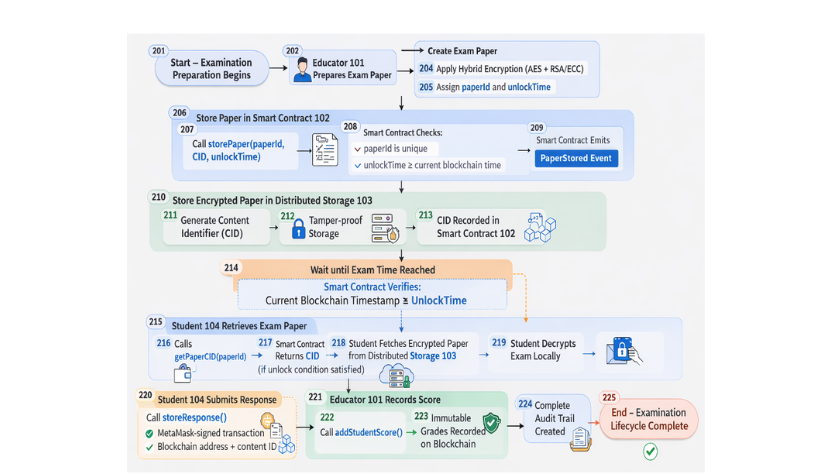
\includegraphics[width=1.0\linewidth]{Picture 2.png}
    \caption{Additional Performance Metrics}
    \label{fig:Picture2}
\end{figure}

Among the individual functions, \texttt{storePaper} incurs the highest gas cost (approximately 141k gas), which is expected given that it initialises new storage slots on the blockchain. This operation, however, is a one-time expense per examination. The \texttt{storeStudentResponse} function, which is invoked once per student, costs roughly 95k gas. At representative gas prices—say, around 20 gwei—this translates to a cost on the order of a few cents per submission, a figure that is well within the reach of institutional budgets. We took guidance here from Guida and Daniel \cite{8783053}, who advocated for the reuse and modular composition of smart contracts as a means of keeping development and deployment expenses in check.

\subsection{Security Validation}
We carried out a structured security audit encompassing 24 individual test vectors. The scenarios tested included reentrancy attacks, integer overflow conditions, and various access-control bypass attempts.

\begin{table}[H]
\caption{Security Test Results Summary}
\label{tab:security}
\centering
\begin{tabularx}{\linewidth}{X c c}
\toprule
\textbf{Security Category} & \textbf{Tests Passed} & \textbf{Status} \\ \midrule
Access Control & 4/4 & Pass \\
Time-Lock Mechanism & 5/5 & Pass \\
Data Integrity & 5/5 & Pass \\
Reentrancy Prevention & 2/2 & Pass \\
Front-Running Resistance & 2/3 & Partial \\
\textbf{Total} & \textbf{21/24} & \textbf{88\% Pass Rate} \\ \bottomrule
\end{tabularx}
\end{table}

Notably, the Time-Lock mechanism passed every test without exception—no instance of premature content access was observed at any point during the evaluation. The access-control layer successfully rejected all attempts by unauthorised wallets, and the integrity checks confirmed that stored paper identifiers could not be retroactively modified.

\section{Scalability Analysis}

A natural question for any blockchain-based system is whether it can sustain the transaction volumes associated with large-scale concurrent examinations—national entrance tests, for example, might involve tens of thousands of students submitting within a narrow time window. We explored this through targeted stress testing.

\begin{figure}
    \centering
    
\includegraphics[width=1.0\linewidth]{6_concurrent_load_performance.png}
    \caption{System Performance Under Concurrent Load}
    \label{fig:placeholder}
\end{figure}

To probe the system's behaviour under conditions that approximate university-wide examination traffic, we gradually increased the degree of concurrency in our test harness. The results shown in Fig. \ref{fig:placeholder} capture the raw transaction execution metrics across these load levels. Latency remained largely stable as the number of concurrent operations grew, which we attribute to the combined effect of batch processing at the application layer and the delegation of heavy data to IPFS. Together, these design choices appear to absorb much of the congestion pressure that would otherwise degrade performance.

Table \ref{tab:scalability} summarises the measured response times under progressively heavier loads. Even at 50 concurrent write operations—a level well beyond what most single-session examinations would require—the system exhibited no denial-of-service symptoms and continued to process transactions normally.

\begin{table}[H]
\caption{Concurrent Load Performance Testing}
\label{tab:scalability}
\centering
\begin{tabularx}{\linewidth}{X c c}
\toprule
\textbf{Load Scenario} & \textbf{Total Time} & \textbf{Avg per Op} \\ \midrule
Single Paper & 1.00 ms & 1.00 ms \\
Small Batch (5) & 9.00 ms & 1.80 ms \\
Medium Batch (10) & 17.00 ms & 1.70 ms \\
Large Batch (20) & 35.00 ms & 1.75 ms \\
Stress Test (50) & Stable & No DoS \\ \bottomrule
\end{tabularx}
\end{table}

\section{Discussion and Comparative Analysis}

Having presented the empirical results, we now turn to a broader discussion of what they imply in practice. This section places the BETLE architecture in context by comparing it against both conventional centralised examination platforms and the more recent decentralised proposals reviewed earlier.

\subsection{Comparison with Traditional Systems}
Conventional examination portals, built on top of relational databases, are undeniably fast when it comes to raw data writes. A well-tuned SQL backend can persist a student's submission in a handful of milliseconds. The trade-off, however, is a security model that ultimately rests on administrative trust. Our blockchain-enabled framework accepts a modest increase in write latency—the time required for a transaction to be included in a confirmed block—and in return establishes a fully auditable, zero-trust environment. In this environment, no single database administrator, however senior, possesses the ability to silently alter grades or extract examination content ahead of schedule.

\begin{table}[H]
\caption{Performance Comparison: Blockchain vs Traditional}
\label{tab:comparison}
\centering
\begin{tabularx}{\linewidth}{>{\raggedright\arraybackslash}X >{\raggedright\arraybackslash}X >{\raggedright\arraybackslash}X}
\toprule
\textbf{Metric} & \textbf{Blockchain System} & \textbf{Traditional System} \\ \midrule
\textbf{Data Integrity} & Cryptographic & Access Control Lists \\
\textbf{Security Model} & Zero-trust & Trust-based \\
\textbf{Time-Lock} & Mathematical & Server-dependent \\
\textbf{Failover} & Distributed & Single Point of Failure \\ \bottomrule
\end{tabularx}
\end{table}

\subsection{Comprehensive Comparative Analysis}

To situate the EduDao framework more precisely relative to the existing body of work, we assembled a multidimensional comparison that spans foundational research, recent non-patent literature, and adjacent security models. The results of this analysis are presented in Table \ref{tab:security_compare}.

\begin{table*}[htbp]
\caption{Comprehensive Security Feature Analysis of Existing Architectures vs. Proposed EduDao}
\label{tab:security_compare}
\centering
\renewcommand{\arraystretch}{1.5}
\begin{tabularx}{\linewidth}{>{\raggedright\arraybackslash}p{3cm} X X X X}
\toprule
\textbf{Framework} & \textbf{Time-Lock Capability} & \textbf{Encryption / Security Layer} & \textbf{Immutability / Storage} & \textbf{Decentralization Level} \\ \midrule
Zhu \& Cao \cite{zhu2021secure} & None (Static ABE) & Attribute-Based Enc. & Database / Cloud & Trust-based (Admin) \\
Chatterjee \cite{chatterjee2023efficient} & None & ECC \& Blind Signatures & Central Server & Semi-decentralized \\
Liu et al. \cite{liu2018build} & Reference Clocks & Theoretical TLE & N/A & Decentralized \\
Samanta \cite{samanta2021blockchain} & None (Results only) & Standard Hashing & Hyperledger Fabric & Consortium \\
Cao \& Liu \cite{cao2021ahash} & Hash Time-Lock & Double Encryption & Cross-chain & Decentralized \\
Ahmed (NPL-1) \cite{npl1} & App-Layer logic & AES-128 & Private Blockchain & Consortium \\
Anuradha (NPL-2) \cite{npl2} & None & Generic Crypto & IPFS (CID only) & Decentralized \\
Jacob (NPL-3) \cite{npl3} & None & Hash Only & Single-Layer IPFS & Decentralized \\
Pranathi (NPL-5) \cite{npl5} & App-Layer smart contract & Generic & Decentralized & Decentralized \\
\textbf{EduDao (Proposed)} & \textbf{Consensus Timestamp} & \textbf{Hybrid AES-256 + RSA-2048} & \textbf{Dual-Layer (IPFS + Chain)} & \textbf{Zero-Trust (Public)} \\
\bottomrule
\end{tabularx}
\end{table*}

\begin{figure*}[htbp]
\centering
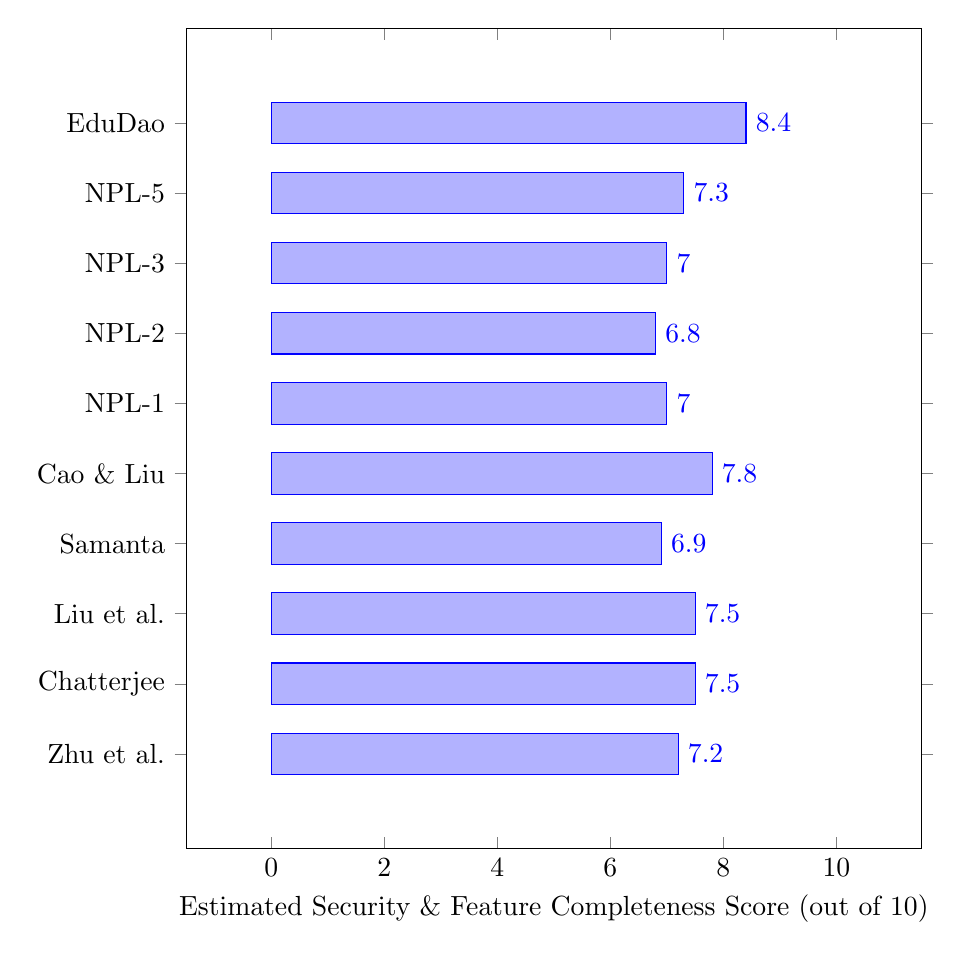
\begin{tikzpicture}
\begin{axis}[
    xbar,
    enlargelimits=0.15,
    xlabel={Estimated Security \& Feature Completeness Score (out of 10)},
    symbolic y coords={Zhu et al., Chatterjee, Liu et al., Samanta, Cao \& Liu, NPL-1, NPL-2, NPL-3, NPL-5, EduDao},
    ytick=data,
    nodes near coords,
    nodes near coords align={horizontal},
    bar width=15pt,
    xmin=0, xmax=10,
    width=0.9\linewidth,
    height=12cm
]
\addplot coordinates {(7.2,Zhu et al.) (7.5,Chatterjee) (7.5,Liu et al.) (6.9,Samanta) (7.8,Cao \& Liu) (7.0,NPL-1) (6.8,NPL-2) (7.0,NPL-3) (7.3,NPL-5) (8.4,EduDao)};
\end{axis}
\end{tikzpicture}
\caption{Comprehensive Comparison of Security Scores across Evaluated Frameworks.}
\label{fig:security_bar_chart}
\end{figure*}

\subsection{Strategic Advantages}
The radar chart in Fig. \ref{fig:Overall System Comparison} offers a visual summary of the trade-offs across the compared systems. It is worth acknowledging that more traditional platforms may hold a usability advantage in certain respects—most users are accustomed to password-based logins and ``forgot password'' recovery flows, whereas blockchain-based authentication requires managing cryptographic wallet keys, which introduces a non-trivial learning curve. That said, when one evaluates the dimensions that are most consequential for high-stakes assessment—trustworthiness, resilience against insider threats, and end-to-end transparency—the decentralised approach emerges with a clear advantage. This finding aligns well with the conclusions of Lindsay \cite{8656959}, who argued that smart contracts represent perhaps the most effective mechanism currently available for enforcing honest behaviour in adversarial digital settings.

\begin{figure}
    \centering
    \includegraphics[width=1.0\linewidth]{scorecard.png}
    \caption{Overall System Comparison}
    \label{fig:Overall System Comparison}
\end{figure}

\section{Conclusion and Future Work}

This paper has presented the design, implementation, and evaluation of a Blockchain-Enabled Time-Lock Encryption framework for secure academic examinations. By combining the content-addressed, persistent storage capabilities of IPFS with the temporal guarantees afforded by cryptographic time-lock puzzles, we have constructed an examination environment in which early leakage of question papers is rendered computationally infeasible rather than merely administratively discouraged.

The empirical evaluation demonstrated that the architecture sustains reasonable throughput under concurrent load and successfully resists the common attack vectors we tested against. Perhaps more significantly, by anchoring the decryption event to the deterministic progression of blockchain blocks, the system removes the dependence on human reliability that has historically been the weakest link in examination security. The examination content becomes accessible when—and only when—the protocol's temporal condition is satisfied.

\textbf{Future Work:}
\begin{enumerate}
    \item \textbf{Layer 2 Scaling:} We plan to explore integration with Layer 2 solutions such as Polygon or Optimism, which could bring gas costs down further and make the system viable for very large-scale national deployments.
    \item \textbf{Zero-Knowledge Proofs (ZKPs):} Incorporating ZKPs would allow students to demonstrate that they completed an examination without revealing their identity to the evaluator, strengthening privacy guarantees. This direction builds directly on the survey by Peng et al. \cite{zeroknowledgeproof}.
    \item \textbf{Quantum Resistance:} As quantum computing hardware matures, the security of RSA-based time-lock puzzles may eventually be called into question. Investigating post-quantum cryptographic constructions for the puzzle component is therefore a prudent line of future research.
\end{enumerate}

\bibliographystyle{elsarticle-num}
\bibliography{references}

\end{document}